\documentclass[11pt]{article}
\usepackage{multicol,graphicx,float,tikz,tikz-qtree,scrextend,apacite,amsbsy,inputenc,amsmath,amssymb,listings,booktabs}
\usepackage[margin=0.7 in]{geometry}
\title{A Method for Analysing Heterogeneous Data with 2D Detection Function Distance Sampling}
\date{January 2018}
\author{Calliste Fagard-Jenkin}
\inputencoding{utf8}

\begin{document}

\lstset{language=R,keywordstyle=\color{blue},stringstyle=\color{green},commentstyle=\color{brown}}
\pagenumbering{gobble}
\maketitle
\begin{center}

\includegraphics[scale=1]{Logo}
\end{center}


\newpage
\emph{I  certify  that  this  project  report  has  been  written  by  me,  is  a  record  of  work  carried  out  by  me,  and  is essentially different from work undertaken for any other purpose or assessment.}

\tableofcontents
\pagenumbering{arabic}
\newpage
\begin{multicols}{2}

\newpage

\section{Abstract}
This project focuses on line-transect distance sampling; a hybrid method which uses both design and model based inference to produce estimates on the sizes of animal populations. An extension of distance sampling by \cite{Borchers} allows for the use of 2D detection functions, describing the probability of detection of an animal in both forward and perpendicular directions. This methodology produces estimates of abundance which are far less biased when compared to estimates produced by conventional distance sampling, when the animals in the population of interest display responsive movement. The raison d'être of this project is to further extend the code-base of the \cite{Borchers} methodology's R package (called LT2D) to include the possibility of covariate inclusion to cope with data that are heterogeneous with respect to detection probability, and to provide a number of illustrative analyses on a range of simulated datasets to demonstrate the improved functionality.

\subsection{Intended readership and summary of objectives}
This project focuses heavily on computation within statistical ecology. Good knowledge of undergraduate statistics is preferable in order to understand the contents. Ideally the reader also has an understanding of animal abundance estimation (specifically distance sampling) and has experience analysing and handling datasets which include covariates. These prerequisites can be summarised by a level of statistical knowledge contained within the MT3507 and MT3508 modules, with knowledge of content within the MT5751 module being ideal.

The intended demographic of readers is researchers in ecological statistics, as well as ecologists who will benefit from reading the latter sections of the project in order to learn how to use the new LT2D software to perform 2D detection function distance sampling analyses on data which display responsive movement with respect to observers, as well as heterogeneity with respect to detection probability. 

This project includes sections which encapsulate computer-theoretic as well as purely statistical content, in order to explain issues of software design, implementation and consideration of user interaction. This is done both to give the reader an in-depth appreciation of how the project achieved its desired outcomes and also to reflect the distribution of work hours the project required. The code-base being modified as part of this project is substantial and complicated, and therefore any implementation of added functionality requires a significant time commitment.

succinctly, the aim of this project is to implement covariate inclusion into the hazard detection functions in the LT2D package resulting from \cite{Borchers}, to add a bootstrap measure of uncertainty on estimates of abundance into the package, to modify goodness of fit and plotting functions to handle covariate-including models and to provide example analyses of simulated data to provide ecologists with knowledge on how to analyse their own data with the new package.

\section{Introduction}
\subsection{Context and background}


\subsubsection{What is distance sampling?}

Distance sampling is a methodology within ecological statistics which allows us to produce unbiased estimates of animal population sizes even when the detection of any individual in the survey area is uncertain. First, a quick description of its simpler alternative, strip sampling (in which detection of individuals is certain), will be given in order to illustrate the fundamental principles of greatest importance. 

Consider a survey area within which the population of interest is closed (there is no emigration or immigration of individuals). We further assume that births and deaths are considered to occur at a negligible rate throughout the duration of the survey. In this way, the survey is considered to be a snapshot of the population at some given moment. In our example, we choose a square survey area, which we subdivide into five strips of regular width. We must further assume that animals are uniformly distributed throughout the survey area, in both the perpendicular and the horizontal axis (in fact, we must simply assume that the distribution of animals with respect to the transect is known. Uniformity arises as a natural consequence of independently distributed transect lines in conventional distance sampling. In the case of point transect distance sampling, the assumed distribution is triangular). The below figure illustrates uniformly distributed animals within a survey area.

\begin{figure}[H]
\centering
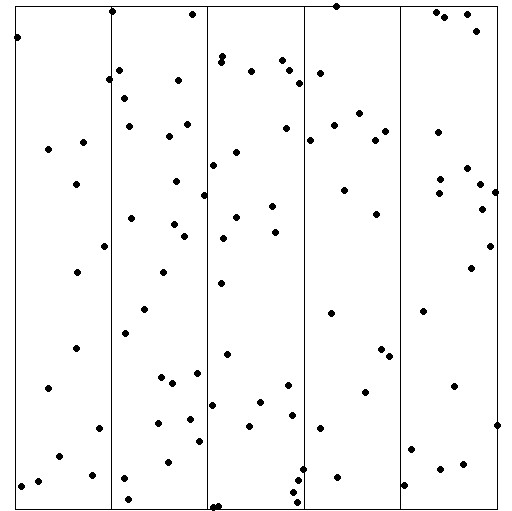
\includegraphics[scale=0.5]{StripSampling}
\caption{Example distribution of animals in a square survey area divided into 5 equal strips}
\end{figure}

Given this rather simplistic design, obtaining an estimate of abundance in the survey area ($\hat{N}$) is extremely simple, so long as we are able to sample all of the individuals within whole strips. As an example we consider strips 2 and 4 (from the left) as the randomly selected strips which form our survey sample. Strip 2 contains 25 individuals, and strip 4 contains 15, giving us a total of $n=40$ observed individuals. If we denote the total survey area by $A$ and the sampled area by $a$, then we observe that our survey effort of $\frac{a}{A}=\frac{2}{5}$. Hence a reasonable intuitive estimator for the abundance in the whole survey area is

\begin{equation}
\hat{N}=\frac{n}{\frac{a}{A}}=\frac{40}{0.4}=100
\end{equation}

which is a simple rescaling of the number of observed animals which accounts for the portion of the survey area which has remained unseen. This example forms a basic overview of an easy methodology we can use when detection of every individual is guaranteed. We would now like to find a way of relaxing the unrealistic assumption of perfect detection. If we assume all animals in the strip have some fixed probability $p$ of being detected, then we can modify our estimator to account for the animals we expect we have missed:

\begin{equation}
\hat{N}=\frac{n}{\frac{a}{A}p}
\end{equation} 


This again is nothing more than rescaling the estimate by an appropriate constant, to account for animals that we believe were present, but not detected by any observers. 


The real hard work begins when we start to ask ourselves how we can estimate this value of average detection probability, which turns out not to be so simple. However, distance sampling comes to the rescue!  In line transect distance sampling, one or multiple observers travel along a transect line which has been pre-determined by the experimental design. Observers look to the left and right of the line as they travel along its path (either on foot, by plane, boat, car etc) and record the perpendicular distance at which each observed animal was detected. Once we pool together all these perpendicular distances for all detected animals, we expect to see a histogram similar to figure 2, which clearly displays that the frequency of detection drops as perpendicular distance increases. This trend has an obvious explanation, owing to the fact that animals become harder and harder to see the farther away they find themselves from the observer(s).

\begin{figure}[H]
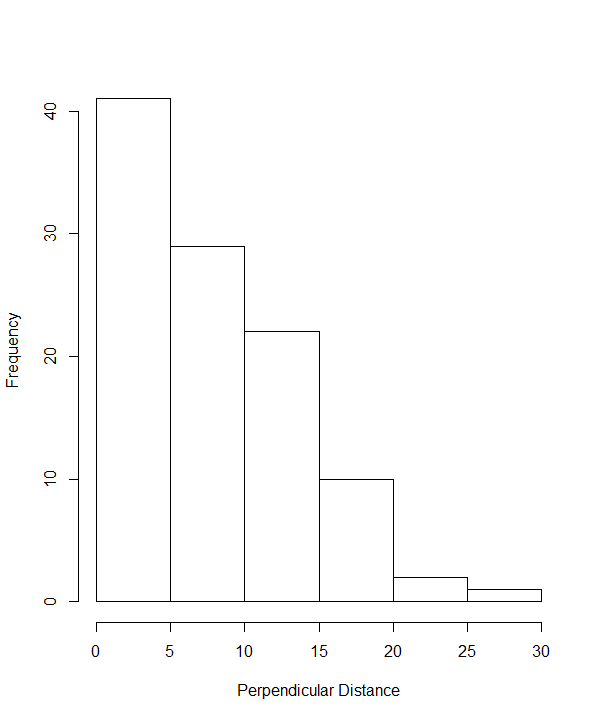
\includegraphics[scale=0.5]{DistanceHist}
\caption{Histogram of perpendicular distances of detected animals}
\end{figure}


A model-based approach which involves the fitting of a detection function, allows us to estimate the way in which perpendicular distance affects detection probability. Figure 3 illustrates this by overlaying a (scaled) half-normal detection function over simulated detection data. Over the course of an analysis, multiple detection functions will be fitted to the data and the most appropriate one selected. In the case of the Distance package written and maintained by the Centre for Research into Ecological and Environmental Modelling, Saint Andrews, this is done by the numerical computation of maximum likelihood estimates of the detection function parameters, and model selection is determined by goodness-of-fit tests as well as information criteria such as Akaike's Information Criterion.


If we momentarily return to the case of perfect detection, we notice that we would expect to see a perfectly flat histogram of perpendicular detection distances (as a result of uniform distribution of animals about the transect line). In this case the bars of our histogram would perfectly cover both the shaded, and un-shaded areas of the large rectangle containing Figure 3. Hence, the ratio of the area under the fitted curve of our detections with respect to the area of this 'perfect detection rectangle' gives us some indication of the average detection probability of the population of interest. In practice, the area of the 'perfect detection rectangle' is extremely easy to calculate (the height of the rectangle is the frequency of detections at perpendicular distance 0, since distance sampling assumes perfect detection on the transect. The width of the rectangle is the perpendicular truncation distance $w$ of the study). The area covered by our own detections is seen as the integral of the detection function over an interval from $0$ to $w$. In order to obtain the sampled area ($a$, in the previous example) in the case of a line transect distance sampling survey, we simply consider $a=2Lw$, where $L$ is the total length of all covered transect lines and $w$ is the previously mentioned perpendicular truncation distance. Thus, with these tools at our disposal, we can modify (2) to obtain:

\begin{equation}
\hat{N}=\frac{n}{\frac{2Lw}{A}\hat{p}}
\end{equation}


where $\hat{p}$ is the estimate of average detection probability we obtain by integrating the detection function and considering the area of the 'perfect detection rectangle'. It should be noted that this description of distance sampling is extremely rudimentary, and is far more intuitive than it is technical. For a deeper understanding of the likelihood functions involved and the design-based, and model-based aspects of the method, reference should be made to both classic and modern literature, such as \cite{EAB} and \cite{DS2015}.

\begin{figure}[H]
\centering
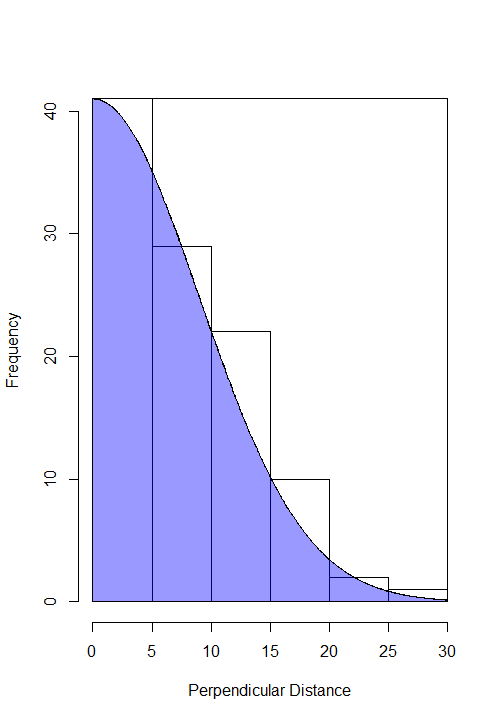
\includegraphics[width=6.38cm]{DistHistDetec}
\caption{Histogram of detection distances with overlayed detection function}
\end{figure}

\subsubsection{The significance of 2D detection functions}

One of the assumptions of distance sampling is that the distribution of animals about the transect line is known. In the previous case of line-transects, it was uniform. Unfortunately, there are many situations in which this assumption is strongly violated, leading to significant bias in estimates of animal abundance and density. One reason for this could be poor survey design, whereby insufficient randomisation of transect line locations leads to trends in the distribution of animals between them. There is no effective analytical solution for poor survey design, and so this case is not considered here. A more interesting cause for this phenomenon is responsive movement of animals in the population of interest. Animals can be scared by observers and hence move away, causing a dip in observed detection frequencies on and close to the transect line, as well a spike in observed detection frequency some relatively small distance away from the transect line. This behaviour is typically referred to as avoidance, and is extremely common in primates, with gibbons being so notoriously prone to the behaviour that they are the subject of regular conventions between ecologists and statisticians. Conversely, animals may also display attraction, whereby an attraction to the transect line causes a spike in detections on the transect line and a dip further out. Dolphins typically display this behaviour when data is collected via shipboard surveys, where the wake of the vessel draws them in.

By considering time-to-detection models, and observing that when an observer is moving along the transect at a constant speed, the forward distance of a detected animal is directly proportional to the time to detection (assuming the animal is stationary), \cite{Borchers} formulate a method by which the relationship between distance and detection probability can be estimated in two-dimensions. This extra information provided in the forward distances of detections also allows the estimation of the perpendicular distributions about the transect line of the detected animals. Once this distribution is known, the issues of responsive movement are largely remedied. It should be noted that the vast majority of studies which collect data which are suitable for the fitting of 2D detection functions often do so by measuring the radial distance to the animal, as well as the angle of incidence of the animal to the observer. Thus the values of perpendicular and forward difference are easily calculated using basic trigonometry. Many of the implementations and intricacies involved with handling edge cases arise directly from this convention and the ways it affects the data and their collection.

\subsection{Previous contributions}

From June - August 2017 I undertook work on the code-base as a summer student at the University of Saint Andrews. The notable changes I made to the code-base over this period will be clearly outlined in this section to distinguish them from the work which was undertaken from September 2017 onward as part of this project, however these will be not be described in depth, in order to avoid removing focus from the more relevant implementations. If more detail on the work conducted in this summer studentship is of interest, it can be found in the slides of a presentation conducted at the 2017 St Andrews Mathematics Undergraduate Research Conference, which have been included in the appendix. 

\subsubsection{Object Oriented Additions}
The R programming language allows for packages to include their own classes to produce objects with behaviours and properties tailored to the task at hand. These typically come in the form of S3 or S4 objects. As part of my summer work I wrote methods for S3 generic functions which allow the LT2D package to be more streamlined and provide the user with a cleaner and more straight forward interface with the functionality provided under the hood. The first set of these methods are dedicated to the R plot function, allowing the user to plot LT2D fitted model objects with a simple call to the generic plot function, with the aforementioned model object as the first argument. 

\subsubsection{Adding in Abundance Estimation}
Previous versions of the code-base only produced estimates for average detection probability, $\hat{p}$. Code supplied by Prof. Borchers was modified and integrated with existing LT2D code to allow the package to produce estimates of abundance as well as average detection probability and effective strip half width. This work was done towards the end of the project and hence was not fully integrated and tested with all other pieces of functionality available within the software, therefore modifications of abundance estimation code and its continual testing and iterative improvement is necessary for the completion of this project, however the details of these updates are of far less interest than the more ambitious aspects of the project and so they shall not be mentioned further in any significant amount of detail. Any addition or modification of code or theoretical technicalities related to the LT2D package mentioned out-with of section 1.2 are not a result of previous work and form the improvements and extensions which the project aims to produce.

\subsubsection{Rounded Angles}
When measurements of small detection angles are rounded down to $0$ in the field, the magnitude of the bias of estimated average detection probability, $\hat{p}$, can drastically increase. An appropriate modification to the method's likelihood function was theorised by prof. Borchers and then I implemented the new functionality into the source code. I conducted multiple simulations to confirm that bias was significantly reduced, all of which clearly demonstrated the new estimator performed far better.

\subsubsection{New Perpendicular Density}
A reparameterisation of an existing perpendicular density was required to allow for a  half-normal perpendicular density function with a non-zero expected frequency of animals on the transect line. Prof. Borchers and I decided on a suitable formulation and I implemented it within the LT2D package. 

\subsubsection{Concatenation of GoF Functions}
Goodness of fit tests (Cramer Von Mises and Kolmogorov-Smirnov) are conducted separately in the x and y (perpendicular and forward) directions, respectively, by the LT2D. These were split into distinct functions, making their use tedious to the end user. I rectified this issue by creating a wrapper function which was easier for the user to interact with and acted as an interface with the pre-existing code.

\subsubsection{Model Collecting and Summarising}
As with many model-based statistical methodologies, it is often good practice to fit a range of varied models to the available data, and to use selection criteria (such as Akaike's Information Criterion) to select which models are most reasonable. This leads to the user's R global environment being peppered with objects created by the LT2D package, making it difficult to keep track of the models of interest. Inspired by another piece of software used for animal abundance (RMARK - An interface to the popular MARK windows software used as a tool for analysis of mark-recapture data) - model-collecting and comparison-table-generating functions were implemented within the LT2D package.

\subsection{Project objectives and outline}
The project aims to include the ability for users to specify covariate inclusion for the two-dimensional detection functions, making them not only a function of perpendicular and forward distance, but also of user-defined relationships between other variables. Upon discussion with Prof. Borchers, it was decided this functionality should be kept as general as possible, following the following main criteria:

\begin{enumerate}
\item Users should be able to choose whether the covariate affects the behaviour of the detection function in the perpendicular direction, the forward direction or at the intercept, or any combination of the above.
\item Users should be able to define the formula which describes the linear predictor for the relevant parameter and the covariate(s) of interest themselves, rather than be restricted to pre-defined options
\item Users should be able to specify different formulas for each parameter (forward, perpendicular and intercept) wherever the detection function allows these to be different.
\item There should be some level of inbuilt error-checking to ensure that users choices for formulas and starting parameter values are consistent between themselves and their choice of detection function
\end{enumerate}

All code calculating estimates of abundance ($\hat{N}$), average detection probability ($\hat{p}$) and AIC should be modified to work with all reasonable choices of covariates and related linear predictors. S3 methods should be written for the plot function to allow it to handle fitted models which contain cases of both discrete and continuous covariate inclusion. The goodness of fit function should also be generalised to use the Kolmogorov-Smirnov and Cramer Von Mises tests when the fitted model has included covariates. The inclusion of code which produces (non-parametric) bootstrap confidence intervals of estimated abundance would also be desirable, for both covariate-including and covariate-excluding models.

\section{Implementation}
\subsection{Covariates; why include them, and how?}
There are many reasons for the desirability of covariate inclusion within the LT2D package. Firstly, when dealing with animal populations which are heterogeneous with respect to detection probability (that is, individuals in the population of interest do not all share a common detection function due to their varying behaviours or characteristics), failing to take this into account often leads to biased estimates of abundance and can even lead to an inability to distinguish amongst reasonable models \cite{Link}, this can be especially prominent in Mark-Recapture analyses, which are the subject of the aforementioned citation. Although distance sampling benefits from the property of pooling robustness, and hence can cope with reasonable levels of heterogeneity within a population \cite{Buckland2004}, 2D detection sampling is based more fundamentally on time-to-detection models and survival analysis, meaning there is no theoretical guarantee that it also shares this robustness with respect to heterogeneous populations. Secondly, we may be interested in performing an analysis on data for which we have associated environmental factors of particular interest. By fitting various models which include different combinations of these covariates, analysing these models' estimated parameters, and by comparing them by standard means of model selection and goodness-of-fit, we may gain insight into the relationship between these covariates and the detection probabilities of individuals within the survey population. Finally, we hope to be able to reduce variance in estimates of abundance and density, by providing more information with which to assess detection probability than the coordinates of detected individuals alone.

We examine the detection functions outlined in \cite{Borchers} and available as part of the associated code-base in order to gain an appreciation for their general form and to ascertain which parameters are most appropriate for covariate inclusion. It should be noted that these detection functions are formulated as hazards of detection, given the location of an animal. Therefore, the terms 'detection function' and 'hazard function' will be used interchangeably henceforth, to allow us to remain consistent with the previous code-base of the LT2D package. Although other, less used hazard functions are present within this code-base, they shall not be examined nor considered for covariate implementation.

%h1
\begingroup
\large

\begin{equation}
h_1\left(y,x;\boldsymbol{\theta}\right) = \theta_1\left(y^2+x^2\right)^{-\frac{\theta_2}{2}}
\end{equation}

%ip1
\begin{equation}
ip_1\left(y,x;\boldsymbol{\theta}\right) = \theta_1\left\{\frac{1}{\sqrt{1+\left(\frac{x}{\theta_2}\right)^2+\left(\frac{y}{\theta_2}\right)^2}}\right\}^{\theta_3 + 1}
\end{equation}

%ip2
\begin{equation}
ip_2\left(y,x;\boldsymbol{\theta}\right) = \theta_1\left\{\frac{1}{\sqrt{1+\left(\frac{x}{\theta_2}\right)^2+\left(\frac{y}{\theta_4}\right)^2}}\right\}^{\theta_3 + 1}
\end{equation}

%ep1

\begin{equation}
ep_1\left(y,x;\boldsymbol{\theta}\right) = \theta_1\left\{\left(\frac{x}{\theta_2}\right)^{\theta_3}+\left(\frac{y}{\theta_2}\right)^{\theta_3}\right\}
\end{equation}

%ep2$
\begin{equation}
ep_2\left(y,x;\boldsymbol{\theta}\right) = \theta_1\left\{\left(\frac{x}{\theta_2}\right)^{\theta_3}+\left(\frac{y}{\theta_4}\right)^{\theta_3}\right\}
\end{equation}
\endgroup

It should be noted that we introduce a log link function to all $\theta$ parameters, in order to allow numerical optimisation routines tasked with finding the maximum likelihood estimates of these parameters the possibility to perform their search anywhere on the real axis. This is with the exception of $ep_1$ and $ep_2$, which use a logit link function for their $\theta_1$ parameters instead.

We notice that all of the above hazard functions share a similar parameter structure. Firstly, they all contain a scale parameter which multiplies the whole function. This is $\theta_1$, which can be interpreted as an 'intercept' for detection probability, given an increase in its value will increase the detection function's value for a given $x$ and $y$, and a reduction in its value will cause the opposite. Secondly, all hazard functions contain parameters which affect the behaviour of the function in the $x$ and $y$ directions. Sometimes the behaviour in both these directions is determined by a single parameter (such as $h_1$, $ip_1$ and $ep_1$, which have both their $x$ and $y$ direction dependent on $\theta_2$), however, in the cases of $ip_2$ and $ep_2$, the inclusion of a $\theta_4$ parameter allows the behaviour in the $y$ direction to be different to that in the $x$ direction.

In the case of $\theta_1$, modifying this parameter to include covariates would enable us to allow for heterogeneity which we believe affects an individual's detection probability, but not the shape of its detection function. In the case of $\theta_2$, covariate inclusion would cause changes in detection function shape in either the $x$ direction alone, or in the $x$ and $y$ directions in the same way, depending on the user's selection of hazard within their model criteria. Any change in $\theta_4$ would cause a change in detection function shape in the $y$ direction alone. We propose the following reformulations of $\theta_1$, $\theta_2$ and $\theta_4$ which allow them to be modelled as the combination of an intercept and a user-specified formula:

\begingroup
\large
\begin{equation}
\mathcal{G}_m\left(\theta_1\right) = \lambda_1 + \mathcal{C}_i\left(\boldsymbol{\gamma}_i\right)
\end{equation}

\begin{equation}
ln\left(\theta_2\right) = \lambda_2 + \mathcal{C}_x\left(\boldsymbol{\gamma}_x\right)
\end{equation}

\begin{equation}
ln\left(\theta_4\right) = \lambda_4 + \mathcal{C}_y\left(\boldsymbol{\gamma}_y\right)
\end{equation}
\endgroup

Where $\mathcal{G}_m$ is the link function appropriate to $\theta_1$ given the detection function given by model specification $m$ the user has selected, $\lambda_1$, $\lambda_2$ and $\lambda_4$ are intercept parameters for the $\theta$ parameter with the corresponding subscript, $\mathcal{C}_i$ is the user specified formula for covariate inclusion in the detection function's intercept, $\mathcal{C}_x$ is the user specified formula for covariate inclusion in the $x$ direction, and $\mathcal{C}_y$ is the user specified formula for covariate inclusion in the $y$ direction. The $\boldsymbol{\gamma}$ are vectors of parameters of the appropriate length required for the corresponding covariate relationship, $\mathcal{C}$. We must have $\mathcal{C}_x=\mathcal{C}_y$ if the detection function specified within model $m$ is $h_1$, $ip_1$ or $ep1$, since $\theta_2$ will affect the detection function's shape in both the $x$ and $y$ directions.

Before considering an example model specification, we introduce the perpendicular density functions within the LT2D package which allow the methodology to account for (and describe) the nature of the observed responsive movement:

\begingroup
\large

\begin{equation}
\pi_U\left(x;\boldsymbol{\phi}\right)=\frac{1}{w}
\end{equation}

\begin{multline}
\pi_{HN}{\left(x;\boldsymbol{\phi}\right)}= e^{-\frac{x^2}{2\phi_1^2}}\left\{\int_0^w{e^{-{\frac{x^2}{2\phi_1^2}}}\ \mathrm{d}x}\right\}^{-1}
\end{multline}

\begin{multline}
\pi_N\left(x;\boldsymbol{\phi}\right)=\\e^{-\frac{\left(x-\phi_2\right)^2}{2\phi_1^2}}\left\{\int_0^w{e^{-\frac{\left(x-\phi_2\right)^2}{2\phi_1^2}}\mathrm{d}x}\right\}^{-1}
\end{multline}

\begin{multline}
\pi_{CN}\left(x;\boldsymbol{\phi}\right) =\\ \left\{1-e^{-\frac{x^2}{2\phi_1^2}}\right\}\left\{w - \int_0^w{e^{-{\frac{x^2}{2\phi_1^2}}}\ \mathrm{d}x}\right\}^{-1}
\end{multline}

\begin{multline}
\pi_{CNi}\left(x;\boldsymbol{\phi}\right) = \\ \left\{1-\phi_2e^{-\frac{x^2}{2\phi_1^2}}\right\}\left\{w - \phi_2\int_0^w{e^{-{\frac{x^2}{2\phi_1^2}}}\ \mathrm{d}x}\right\}^{-1}
\end{multline}
\endgroup

$\pi_U$ reflects the assumption of no responsive movement, whereas $\pi_{HN}$ reflects the assumption that animals we be attracted to the transect line and $\pi_{CN}$ reflects the assumption that animals will display avoidance. $\pi_N$ is flexible enough to model both attraction and avoidance. \cite{Borchers}. $\pi_{CNi}$ is a reparameterisation of $\pi_{CN}$ which allows for non-zero expected abundance on the transect line.

For illustration, we now consider an example model $m$ specified by a user of the LT2D package, which selects an $ip_2$ detection function as well as a $\pi_{HN}$ perpendicular density distribution. Data collected by the user includes all of the standard information required to perform an estimate of abundance through conventional distance sampling (CDS), as well as the forward distance of each detection, a factor covariate $species$ (with three levels), a continuous covariate $forest.cover$ and another continuous covariate $size$, which for each detection refers to the number of individuals in the detected group. The user has specified that the $i$ direction (the intercept) should include the relationship $i\sim forest.cover$ (using R tilde notation for the specification of formulas). The user would also like to assume that $x\sim species$ and $y\sim size$ to specify the nature of covariate inclusion in the $x$ and $y$ directions respectively. Given this, the full formula for the detection function is given by:

\begin{multline}
hr_m\left(y,x;\boldsymbol{\theta}\right) = \theta_1\left\{\frac{1}{\sqrt{1+\left(\frac{x}{\theta_2}\right)^2+\left(\frac{y}{\theta_4}\right)^2}}\right\}^{\theta_3 + 1}\\\theta_1=exp\left\{{\lambda_1 + \gamma_{1,1}forest.cover_{y,x}}\right\} \\\theta_2 = exp\{\lambda_2 + \mathcal{I}_2\left(species_{y,x}\right)\gamma_{2,1}\\ +\mathcal{I}_3\left(species_{y,x}\right)\gamma_{2,2}\}  \\\theta_4 = exp\left\{\lambda_4 + \gamma_{4,1}size_{y,x}\right\}
\end{multline}

With equation (13) perpendicular density function. Where $hr_m$ represents the hazard detection function corresponding to the model specification m and the $\lambda$ parameters are intercepts for the corresponding $\theta$ parameters. $forest.cover_{y,x}$, $species_{y,x}$, and $size_{y,x}$ are the values of $forest.cover$, $species$ and $size$ respectively, for the detection at coordinate $(x,y)$.

It becomes clear that allowing the user a selection of choices for covariate inclusion with complete freedom of choice for formulas as well as which detections function to select, which perpendicular density function to select, and allowing each parameter to have a different formula quickly becomes an issue of not only statistical theory, but also a problem rooted in software design. We must construct a general methodology which allows users to specify in simple terms the model specification they desire, with software capable of producing the corresponding design matrices and linear predictors whilst also being able to error-check the user's inputs for inconsistency. For example, a user attempting to fit different covariate formulas in the $x$ and $y$ directions when hazard function $h_1$ is selected should raise an error, since this detection function is not flexible enough to allow this. The following section provides an insight into the choices made to achieve the implementation of the above described functionality. Individuals primarily concerned with learning how to use the new LT2D software to produce analyses on their own data should feel free to skip to chapter 4.

\subsection{Understanding the LT2D software and its architecture}
In order to implement covariate inclusion it is vital to first understand the inner workings of the LT2D package, so that we may ascertain both the complexity of the task at hand, and also the most efficient method with which to proceed. A simplification of the software's top-level fitting function call hierarchy (as of August 2017, before the project began), which retains the features of greatest importance and relevance is illustrated by figure 4.

\begin{figure}[H]
% the following code was used to produce the image. It was then exported as an image and then reincluded into the document as a static to allow for easier resizing
%\begin{tikzpicture}[scale=1.5]
%\Tree[.LT2D.fit [.fityx [.optim [.negloglik.yx [.p.pi.x [.pi.x ]  [.px [.Sy [.hr ] [.pi.x ] ] ] ] [.fyx [.hr ]  ] ] ] [.solve ] ][.NDest  [.invp1\_replacement [.phat [.hr ] [.pi.x ] ] ] ] ]
%\end{tikzpicture}
\centering
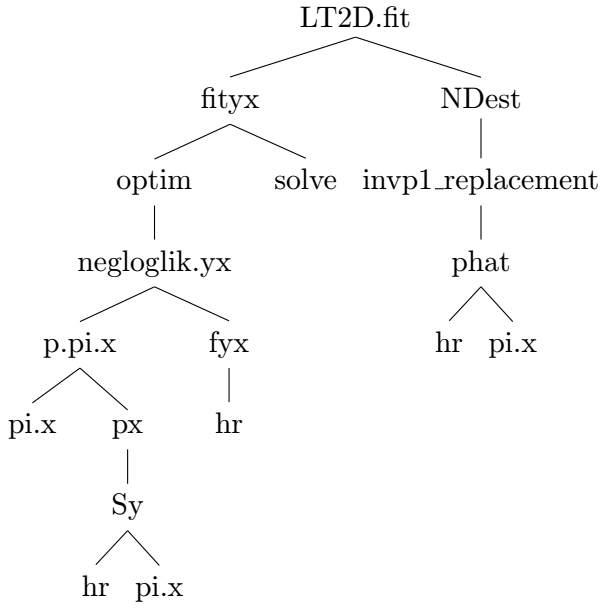
\includegraphics[scale=0.507]{LT2Dprecov}
\caption{Simplified call hierarchy for the top-level fitting function in the LT2D software}
\end{figure}
This diagram illustrates the inner workings of the LT2D package in slightly more detail than the description given by \cite{Borchers}. Below, a brief outline and description of each of the functions in figure 4 will be given to give the reader a general understanding of how the LT2D package used to fit models to data before covariate implementation, and how it evaluates the likelihood function outlined in \cite{Borchers}:

\begin{itemize}
\item LT2D.fit ; A function which given an appropriate input R data.frame and model specification settings, produces a two-dimensional detection function distance sampling maximum likelihood estimation of model parameters and abundance.

\item fityx ; The function responsible for the model-fitting provided by LT2D.fit.

\item NDest ; The function tasked with calculating estimates of abundance and density, when provided with the output of the fityx function.

\item optim ; The linear optimisation routine which provides maximum likelihood estimation of the model parameters.

\item solve ; The function which solves the hessian matrix provided by optim in order to produce a variance-covariance matrix for the estimated parameters.

\item invp1\_replacement ; The function which produces an estimate of inverse effective half strip width, given the chosen model settings and their estimated parameters.

\item negloglik.yx ; The function which evaluates the negative log likelihood - the probability of observing the observations we saw, given the model specifications and their estimated parameters.

\item phat ; The function tasked with calculating effective half strip width, given model specifications and their estimated parameters.

\item p.pi.x ; The function which evaluates the product of the probability of detection at a given perpendicular distance and the probability of an animal's presence at that perpendicular distance, given model specifications and their estimated parameters.

\item fyx ; Calculates the probability density function of the 'waiting distance', given model specifications and their estimated parameters.

\item hr ; Evaluates the two-dimensional detection function specified by the user as part of the model specification. Returns the hazard rate of detection given estimated parameters.

\item pi.x ; Evaluates the assumed perpendicular density distribution of animals about the transect line, selected by the user. Returns the probability of the animal's location at a given perpendicular distance given estimated parameters.

\item px ; Numerically calculates the perpendicular detection function from a specification of a hazard function (in the form of hr, above) and its estimated parameters.

\item Sy ; Calculates the survivor function to a given forward distance. Evaluates the probability of an animal remaining undetected until a given forward distance ahead of the observer, and then being detected at that distance, given model specifications and their estimated parameters.
\end{itemize}

\subsection{Implementation of covariates into the likelihood}
Fundamentally, an implementation of covariate inclusion requires the conversion of a model specification into a set of design matrices and corresponding linear predictors for the $\theta$ parameters of the user-selected detection function. For computational efficiency, we wish to perform this conversion as infrequently as possible. Because of this, performing these calculations at the lowest level of the tree illustrated by figure 4 is extremely wasteful, owing to the fact that at every evaluation of the detection function, we must recalculate the set of design matrices and corresponding linear predictors, and that the detection function may be called many times by any function which is only a single level above it in the figure 4 tree. To achieve optimal efficiency, we must perform the conversion calculations as high up the figure 4 tree as is possible, so that the results of these calculations can simply 'trickle down' the tree, rather than have to be recalculated at every step.

The design matrices depend only the user selected formulas, and so can be calculated as soon as the LT2D.fit function passes the information which constitutes the model specification to the fitting function fityx. For this reason, all design matrices are calculated within fityx, as this is the highest level in the tree which has access to all the required information, whilst remaining modular enough a solution to leave the top-level function as streamlined as possible. The linear predictors however - which calculate the $\theta$ values of the detection function, given a set of estimated parameters - depend on not only the design matrices, but also the set of estimated $\lambda$ and $\gamma$ parameters estimated by the current iteration of the numerical optimisation. Because of this dependency, we must calculate the linear predictors below the level in which optim resides in figure 4. Therefore, the highest point in the tree we can calculate linear predictors is inside the negloglik.yx function itself. 

% the following code was used to produce the image. It was then exported as an image and then reincluded into the document as a static to allow for easier resizing
%\begin{tikzpicture}[scale=1.5, level distance=50]
%\Tree[.fityx [.HazardCovarSlots ] [.FormulaChecking [.HazardCovarsAllowed ] ] [.DesignMatrix ] [.unlist ] [.optim ] ]
%\end{tikzpicture}

\begin{figure}[H]
\center
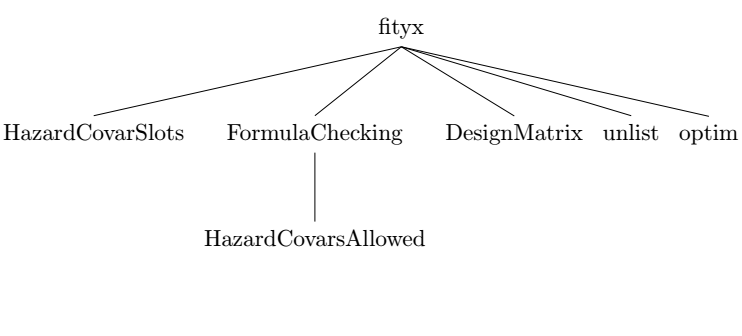
\includegraphics[scale=0.4512]{LT2Dpostcovfityx}
\caption{Simplified call hierarchy for fityx after covariate inclusion}
\end{figure}

%\begin{tikzpicture}[scale=2.5]
%\Tree[.optim [.negloglik.yx [.p.pi.x [.pi.x ] [.px [.Sy [.hr ] [.pi.x ] ] ] ] [.fyx [.hr ] ] [.relist ] [.LinPredictor ] ] ]
%\end{tikzpicture}

\begin{figure}[H]
\center
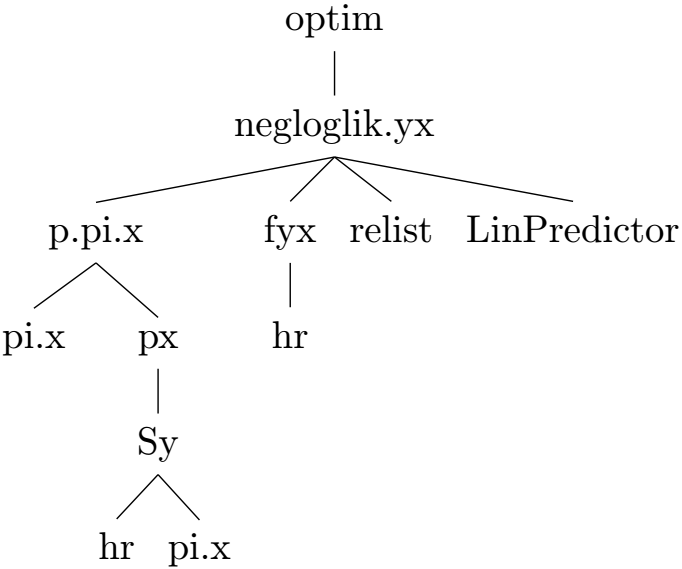
\includegraphics[scale=0.4909]{LT2Dpostcovoptim}
\caption{Simplified call hierarchy for optim after covariate inclusion}
\end{figure}

Functions which perform these conversion calculations, error-check user choices of covariate formulas and model selection specifications as well as provide an interface with optim which allows the LT2D.fit function to be used for both covariate-including and covariate-excluding models were implemented and lead to the fityx call hierarchy becoming that which is illustrated by figures 5 and 6. 

The call to the solve function is still present, but has been omitted from the diagram in the interest of simplicity and space. Post covariate implementation, detection functions now require their parameters to be given as an R list, as opposed to a vector (this allows us to provide a separate set of parameters for each detection). Elements in these lists will be referred to as 'slots' to avoid confusing them with 'elements' within R vectors. 

HazardCovarSlots is a function which indicates to fityx which slots within the input list of $\theta$s are able to be turned into a linear predictor, depending on the user-selected detection function. FormulaChecking is a function which raises an error if the user has specified formulas incorrectly, or in a way which is not compatible with the detection function they have chosen. DesignMatrix produces the appropriate design matrix for a $\theta$  parameter, given the user-specified formula and the R data.frame which contains both the user's data and the covariates referred to in the covariate formula. unlist converts the list of $\theta$ parameters into a vector, since this is the only type of input allowed by the numerical optimisation routine 'optim'. Looking at figure 6 to further detail optim's call hierarchy with covariates implemented, we notice the addition of the relist function, which converts optim's vector of estimated parameters back into the list structure they were in previous to being passed to optim, and the function LinPredictor which uses the optim estimates and the design matrices calculated by fityx to produce the $\theta$ parameters for the detection function.

The vast majority of functions within the fityx call hierarchy had to be modified and generalised to handle each detection having different estimated $\theta$ values for the same detection function. In many cases this had to involve the introduction of 'for' loops to produce a calculation separately for each detection, which represents part of the computational overhead required for giving the user the possibility to deal with  heterogeneous data. The other significant overheads being the calculation of design matrices, linear predictors and the estimation of multiple new parameters by the numerical optimisation routine.  

\subsection{Covariate inclusion into abundance estimation}
The function $invp1\_replacement$ needed to be modified to calculate separate estimates of effective strip half-width for each detection, given that with covariate-included models, we expect the estimated $\theta$ parameters to be different for all detections which do not share identical covariate values. This involved making individual calls to the $phat$ function to obtain the estimate of effective strip half width for each detection.

If analyses on large datasets are required, it could be worth implementing a procedure which attempts to evaluate how many different covariate combinations are present within the data, and to produce a call to $phat$ for each of these once, rather than for each detection separately (which makes no consideration of whether or not a calculation has already been made for a detection with the same covariate values). This optimisation is likely to only be noticeable in the presence of factor covariates within large data sets, given that this scenario leads to the highest possible frequency of repeated covariate values between detections.

\subsection{Modification of goodness of fit functions}
The LT2D goodness of fit methodology divides the goodness of fit into separate calculations for the perpendicular and forward distances of detections. Aside from the modifications made to incorporate covariate-included goodness-of-fit, the goodness of fit functionality was already integrated into the LT2D package at the time of publication of \cite{Borchers}.

In the $y$ direction, the test is performed by considering the CDF of the conditional survival function of detections, compared with the empirical CDF of the same function. For example, for a collection of detections, and for each detection within these, we consider the probability of the animal 'surviving' (remaining undetected) until its forward distance of detection $y$, and we call this probability $p$. $1-p$ is then the probability that this animal does not survive any further than forward distance $y$. We also denote by $1-p_0$ the probability that the animal does not survive all the way to the observer (at forward distance $y=0$). Hence by          considering the conditional probability $\mathbb{P}\left(A|B\right) = \frac{\mathbb{P}\left(A\cap B\right)}{\mathbb{P}\left(B\right)}$ and noticing that the probability of not surviving past $y$ whilst also not surviving past $0$ is simply the probability of not survivng past $y$, we can determine that the probability of not-surviving past $y$ given that the animal did not survive further than the forward distance of the observer ($0$), is $\frac{1-p}{1-p_0}$. By evaluating the theoretical CDF of conditional survival probability for each detection in this way, and comparing it to the empirical CDF, we obtain enough information to produce a Kolmogorov-Smirnov and Cramer von Mises goodness of fit test in the forward direction. To cope with covariate-included models, we use the fitted $\theta$ values for each individual point to produce the evaluation of $\frac{1-p}{1-p_0}$, rather than using a single set of $\theta$s for the whole data set. 

In the $x$ direction we again consider the conditional CDF of a distribution. For the numerator we consider the probability of an animal being detected between perpendicular distance $0$ and the perpendicular distance $x$ at which its detection took place, given fitted values for both its perpendicular density and detection function. The denominator evaluates the probability of the animal being detected between perpendicular distances $0$ and truncation distance $w$ (the full range of the survey), and hence we obtain the probability of detection within $0$ and the observed perpendicular detection distance $x$, given the animal was detected within the perpendicular survey range (and given the fitted parameters of the model's detection function and perpendicular density function). To account for covariate-included models we again allow this probability to be calculated individually for each point, given its own estimated $\theta$ parameters, and then perform the rest of the test as before. 

\subsection{Implementation of confidence intervals}
Previous to this project, the LT2D package was only able to produce point estimates for abundance, with no measure of uncertainty. Due to the complexity of the 2D detection function distance sampling likelihood, analytical calculation of confidence intervals is infeasible, and therefore we consider the use of a bootstrap. The use of a parametric bootstrap, re-sampling detections from a set of simulations of the fitted detection and perpendicular density functions would allow us to circumvent making any assumptions on the distributions of the fitted maximum likelihood estimates. However, the LT2D software can take several minutes to fit complicated models with many covariates, and therefore obtaining a large enough re-sample size to produce a reasonable bootstrap confidence interval would represent a commitment in computation time which is too elevated to be of practical benefit.  Because of this, we settle on the use of a non-parametric bootstrap which is dependent on the estimated asymptotic distributions of the maximum likelihood estimates, despite these assumptions being somewhat unrealistic when sample sizes are small.  The $LT2D.bootstrap$ function uses information provided in the hessian matrix produced by optim to produce a variance-covariance matrix for the MLEs. A large sample (the size of which can be selected by the user) is then taken from  the multivariate normal distribution centred at the obtained MLEs, with variance-covariance matrix equal to the solved hessian matrix produced by optim. Each of these samples is then converted into a set of $\theta$ and $\phi$ parameters appropriate to the fitted model's covariates, detection function and perpendicular density. These parameters are then passed along with the original data to the $NDest$ function to obtain an estimate of abundance. Once this process has been completed for all generated re-samples, a $(1-\alpha) 100\%$ confidence interval for abundance is produced using the percentile method. 

Due to relatively high parameter sensitivity, small changes in estimated parameters can cause a large change in estimated abundance. This leads to the implemented bootstrap producing intervals that tend to be too wide, resulting in a coverage which is superior the selected value of $(1-\alpha) 100\%$. Although coverage which is better than expected is not of itself undesirable, it highlights that we may be able to produce intervals with a smaller range should we switch to a different methodology, which is something to be considered during further development of the LT2D package. 

\subsection{Modification of plot functions}
The LT2D plot functions required slight modifications in order to be able to handle models with covariates included. Due to the infinite combination of choices of covariate values when these covariates are continuous (and growing according the the factorial of the number of levels for each of the factor level covariates), it was decided that producing plots for all covariate levels or for a fixed proportion of them was not possible. The plotting function therefore allows the user to select the integer number which represents the row of the original R data.frame which contains the detection who's covariate values are to be chosen as the values to be held fixed whilst plotting the various curves the plotting functions produce.  The option to overlay plots for a selection of these, or to manually specify a single set of covariate values which are to be held fixed would be desirable as the LT2D software develops further.

\section{Usage of the new software}
We now provide a selection of illustrative uses of the new LT2D software through the use of simulated data. All the following code is in R, with the LT2D package installed as the version included in the appendix of this project. The detection functions which constitute equations (4) through (8) inclusive are named h1, ip1, 1p2, ep1 and ep2 respectively within the LT2D package. The perpendicular density functions given by equations (12) through (16) inclusive are called pi.const, pi.hnorm, pi.norm, pi.chnorm and pi.chnorm.i respectively. We will begin our example by simulating a collection of detections from a population of size $N=500$, with an h1 detection function and a normal perpendicular density. 

\begingroup
\small
\begin{lstlisting}
library('LT2D')

# set perp trunc, forward trunc
# total transect length and survey
# area:
w = 0.03 ; ystart = 0.05
L = 10 ; A = 2*w*L

# set value of 'true' parameters
# for simulated data:
b <- c(-4.04,0.79)
logphi <- c(0.02,-4.42)

# produce simulated data:
set.seed(3)
simDat = simXY(500, 'pi.norm',
               logphi, 'h1', 
               b, w, 
               ystart)$locs
\end{lstlisting}
\endgroup

Our next task is to put these simulated data into an R data.frame which contains the following categories:

\begin{itemize}
\item x - The $x$-coordinate for each detection. Can have the value NA if no detection was made on the given transect.
\item y - The $y$-coordinate for each detection. Can have the value NA if no detection was made on the given transect.
stratum - The stratum within which the detection was made
\item transect - The transect on which the detection was made
\item L - The total length of the transect on which the detection was made
\item area - The survey area of the stratum within which the detection was made
\item object - The object number of the detection. All detections must have a unique number, this can be set to NA on a transect where no detections were made.
\item size - The number of animals in the group that was detected
\end{itemize}

The below code produces a simulated data.frame with the correct column names and values using the simulated data $simDat$:

\begingroup
\small
\begin{lstlisting}
# create the data.frame:
all.1s <- rep(1,length(simDat$x))
obj <- 1:length(simDat$x)
sim.df <- data.frame(x = simDat$x,
                    y = simDat$y,
                    stratum = all.1s,
                    transect = all.1s,
                    L = L,
                    area = A,
                    object = obj,
                    size = all.1s)
\end{lstlisting}
\endgroup

For the simulated data set sim.df we created above, the first few rows (with some truncation in the x and y values) of the data frame are:

\begin{center}
\tabcolsep=0.07cm
 \begin{tabular}{||c c c c c c c c||} 
 \hline
 x & y & stratum & transect & L & area & object & size\\ [0.5ex] 
 \hline\hline
 0.0050 & 0.0327 & 1 & 1 & 10 & 0.6 & 1 & 1 \\ 
 \hline
 0.0242 & 0.0322 & 1 & 1 & 10 & 0.6 & 2 & 1 \\
 \hline
 0.0115 & 0.0079 & 1 & 1 & 10 & 0.6 & 3 & 1 \\
 \hline
 0.0098 & 0.0305 & 1 & 1 & 10 & 0.6 & 4 & 1 \\
 \hline
 0.0180 & 0.0186 & 1 & 1 & 10 & 0.6 & 5 & 1 \\
 \hline
\end{tabular}
\end{center}

To fit a simple model with no covariate inclusion, we call the LT2D.fit function in the following way:

\begingroup
\small
\begin{lstlisting}
# fit an LT2D model
fit <- LT2D.fit(DataFrameInput = sim.df,
                hr = 'h1',
                # start values for b:
                b = c(-3.72,0.74),
                ystart = ystart,
                pi.x = 'pi.norm',
                # start values for logphi:
                logphi = c(0.02, -4.42),
                w = w,
                hessian = TRUE)
\end{lstlisting}
\endgroup

\begin{figure}[H]
\center
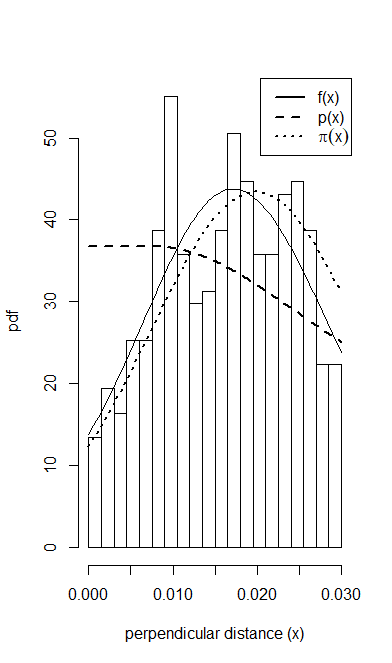
\includegraphics[scale=0.85]{fig7}
\caption{Fitted curves for simulated data in the $x$ direction}
\end{figure}


Calls to the $gof.LT2D$, $LT2D.bootstrap$ and $plot$ functions produce goodness of fit vales for us, calculate a confidence interval on abundance using our chosen number of re-samples and plot the fitted curves. We can also extract the AIC from the fitted model object:

\begingroup
\small
\begin{lstlisting}
gof.LT2D(fit)
LT2D.bootstrap(fit,999)$ci
plot(fit)
fit$fit$AIC
\end{lstlisting}
\endgroup

Which gives us the GoF values:
\begin{center}
 \begin{tabular}{|c c c|} 
 \hline
 \  & KS & CvM \\ [0.5ex] 
 \hline
 X & 0.7130 & 0.7933 \\ 
 \hline
 Y & 0.9429 & 0.9300  \\
 \hline
\end{tabular}
\end{center}


Figures 7 and 8 display the fitted curves the simulated data. The bootstrap results in a 95\% confidence interval of $(490,.88,514.20)$ with 999 re-samples, from $n=448$ detections, with our fitted model producing an estimate of $\hat{N}=503$.  We add in some simulated covariate values to our data frame. We consider a continuous covariate $altitude.sim$ and a factor covariate $observer.id$, it should be noted that we are not further changing the simulated data other than by adding artifical columns into the data.frame that contains them, and so models including these fake covariates are expected to fit poorly. Their inclusion is there solely to illustrate how to specify covariates as part of a model within the LT2D software. The formulas argument to the $LT2D.fit$ function must be a list of R objects with class 'formula'. These are all of the form described in section 3.1. For each formula which is included within the model in this way, a vector of initial guesses must be passed to LT2D.fit, with the name ipars, xpars or ypars, depending on the formula specified. It is possible to specify multiple formulas at the same time, if the choice of detection function allows it (the software returns a warning and sometimes also an error if invalid combinations are selected by the user).

\begingroup
\footnotesize
\begin{lstlisting}
set.seed(3)

n <- length(simDat$x)

sim.df$observer.id <- factor(sample(
  1:3,n,replace=T))

sim.df$altitude <-  rnorm(n,2,1)

iform <- formula(i~sim.df$observer.id)
xform <- formula(x~sim.df$altitude)
yform <- formula(y~sim.df$altitude)
# covariates in intercept only
fit2 <- LT2D.fit(DataFrameInput = sim.df,
                 hr = 'h1',
                 # start values for b:
                 b = c(-3.72,0.74),
                 ystart = ystart,
                 pi.x = 'pi.norm',
                 # start values for logphi:
                 logphi = c(0.02, -4.42),
                 w = w,
                 hessian = TRUE,
                 formulas = list(iform),
                 ipars=rep(0,2))

# covariates in the x and y directions
# (which must have the same effect in 
# an h1 detection function)
fit3 <- LT2D.fit(DataFrameInput = sim.df,
                 hr = 'h1',
                 # start values for b:
                 b = c(-3.72,0.74),
                 ystart = ystart,
                 pi.x = 'pi.norm',
                 # start values for logphi:
                 logphi = c(0.02, -4.42),
                 w = w,
                 hessian = TRUE,
                 formulas=list(xform,yform),
                 xpars=0,
                 ypars=0)

# covariates in all of the h1 slots
fit4 <- LT2D.fit(DataFrameInput = sim.df,
                 hr = 'h1',
                 # start values for b:
                 b = c(-3.72,0.74),
                 ystart = ystart,
                 pi.x = 'pi.norm',
                 # start values for logphi:
                 logphi = c(0.02, -4.42),
                 w = w,
                 hessian = TRUE,
                 formulas=list(iform,
                 		xform,
                 		yform),
                 ipars=0
                 xpars=0,
                 ypars=0)
\end{lstlisting}
\endgroup


\section{Simulation studies}
Producing a simulation study to ascertain the new software's capacity to account for heterogeneous populations is made difficult by a number of factors. Firstly, as the \cite{Borchers} likelihood is complicated and requires multiple instances of numerical integration at every evaluation, model fitting and maximum likelihood estimation takes a significant amount of time. Models which have no covariate inclusion may take only a few seconds to be fitted to a relatively small sample, however, the inclusion of covariates increases this computational cost quite heavily, increasing the quantity of numerical integration involved (by having to evaluate each point individually, due to its own distinct estimated values of the detection function parameters, based on its covariate values) as well as requiring more calls to the likelihood function in order to numerically estimate its maximum likelihood estimates. This causes models with even relatively simple covariate formulas to sometimes take upwards of 15 minutes to compute. Therefore producing a simulation study which includes a large number of fitted models with covariate formulas is understandably difficult.

\begin{figure}[H]
\center
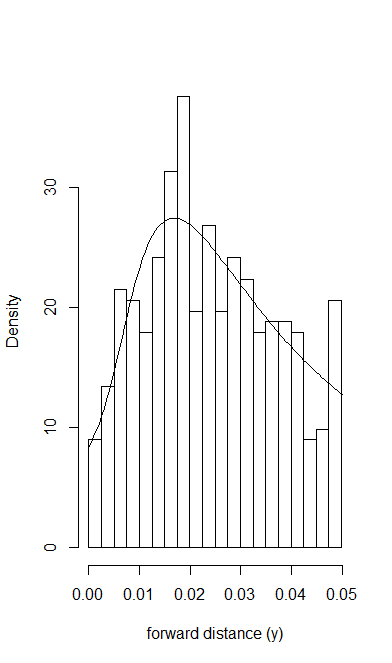
\includegraphics[scale=0.85]{fig8}
\caption{Fitted curves for simulated data in the $y$ direction}
\end{figure}

A second complication arises due to optim's sensitivity to specified starting values for the parameters which are being estimated. The numerical optimisation routine struggles to produce estimates for these parameters when the initial estimates are not close to the 'true' maximum likelihood estimate. This is made visible to the user by a constant sequence of convergence error codes and warnings produced by the optim function, when the initial values were too different from the 'true' parameter values. A common remedy to this problem is to fit a single model multiple times, using the previous iteration's estimated parameters as the set of initial parameter estimates specified within the current model specification. This reduces the difference between the 'true' parameters and the supplied initial values with each iteration, making it easier for optim to converge.

Models which have covariates specified are more prone to this problem, due to their intrinsically more complicated nature. Pilot simulation studies revealed that not being able to manually re-fit models using the previous model's estimated parameters negatively affected covariate-including models more heavily than covariate-excluding models, due to the covariate-including models converging with more difficulty. This difficulty to converge lead to estimates of abundance produced by covariate-including models to be estimated as being far more biased than they would be in practice, as a result of the simulation relying on parameter estimates from poorly converging models to produce its estimates of abundance.

A solution to this problem would be to include an option for the software to automatically recognise poor convergence in maximum likelihood estimates, and to perform a new estimation of the parameters using the previous estimates as initial values. This implementation would be complicated due to the desired flexibility of the covariate inclusion, and so is deemed too substantial to include as part of this project. We are therefore limited to simulation studies with very few fitted models, so that we may manually ensure that convergence for each model is reasonable, and therefore representative of the software's performance in practice. 
\section{Going forwards}
\subsection{Additional desired features}
\subsection{A proposed approach for mixture model incorporation}
\section{Conclusion}
This project's primary aim has been the implementation of covariates within the 2-Dimensional detection functions of the methodology provided by \cite{Borchers}, and to provide this additional functionality within the LT2D package itself, to increase its scope and feature set. The work completed for this project has allowed the LT2D software  to provide flexible methods for the user to deal with data which are heterogeneous with respect to detection probability, with a simple user interface. The user is able to choose any combination of covariates, be they quantitative or qualitative, and is able to specify separate formulas for each direction of the detection function. Plotting and goodness of fit functions have been generalised to be able to handle models with covariates included, with the possibility of calling the plot function multiple times to produce figures of the fitted curves at different levels of the included covariates. Not only has the abundance estimation within the software been generalised to produce point estimates when covariates have been included within a user's selected model, but it has also been extended to produce a bootstrap confidence interval of abundance (with the flexibility for the user to modify both the expected coverage and the bootstrap's  number of re-samples). 

The implementation of this covariate inclusion required intimate knowledge of the \cite{Borchers} paper and the theory which underpins its software, as well as the ability to work with its substantial and complicated pre-existing code base to include the desired additional functionality. A strong grasp of good programming practice, relevant computer theoretic notions and comfort with the R programming language were all required to make the desired changes in an computationally efficient way. The use of techniques and practices outlined in \cite{Hadley} allowed the inclusion of more advanced functionality to the user by making use of R features which go above the scope of undergraduate statistics content (such as object oriented programming, exception handling, etc). 

Due to the feature set of the new software, its flexibility and easy of use, it is my belief that the objectives outlined by this project have been comfortably met. Further examples of the software's use and demonstrations of it's ability to handle general cases can be found in the appendix.

\bibliographystyle{apacite}
\bibliography{Biblio}
\end{multicols}

\section{Appendix}

Given that the LT2D source code is approximately 3500 lines of R code (after the completion of this project), and that the inclusions which constitute this project are over 1500 alone, GitHub links to the relevant files will be included to avoid bloating this document.


The example code included in section 4, as well as an example of the type of code used to produce the pilot simulation studies mentioned in section 5 can be found here: 
\\
\url{https://github.com/penguin-coding/LT2D-work/blob/master/LatexRCode.R}\\

The LT2D functions code before the project:
\\\url{https://github.com/penguin-coding/LT2D-work/blob/master/2DLTfunctions\%20-\%20Copy.r}\\

The LT2D functions after the project:\\\url{
https://github.com/penguin-coding/LT2D-work/blob/master/LT2D/R/2DLTfunctions.r}\\

The LT2D GoF functions after the project:\\
\url{https://github.com/penguin-coding/LT2D-work/blob/master/LT2D/R/2DLTGoF.R}\\

An example of how to fit different covariate formulas to a real data set:\\


\subsection{LT2D code}

\end{document}
